\documentclass[crop,class=article]{standalone}
%----------------------------Preamble-------------------------------%
\usepackage{tikz}                       % Drawing/graphing tools.
\usetikzlibrary{arrows.meta}            % Latex arrows.
%--------------------------Main Document----------------------------%
\begin{document}
    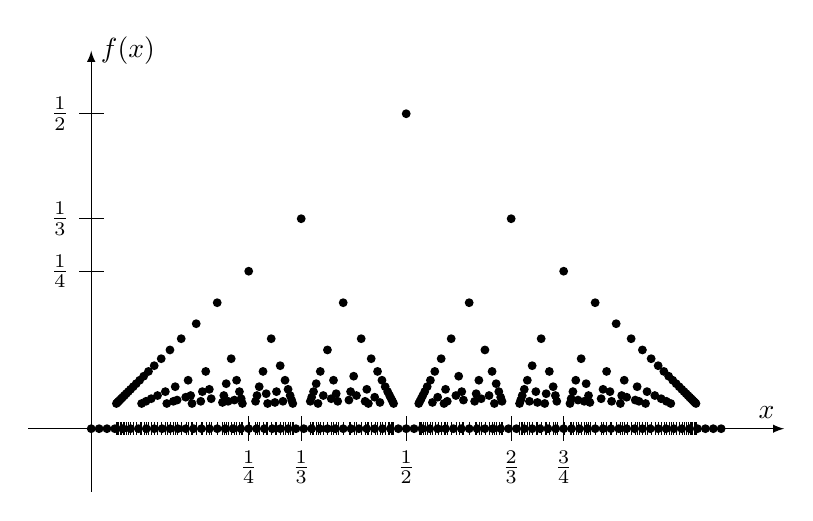
\begin{tikzpicture}[scale=8,>=latex]
        \draw[->] (-0.1,0) -- (1.1,0)
            node[above left] {$x$};
        \draw[->] (0,-0.1) -- (0,0.6)
            node[right] {$f(x)$};
        \draw (0.02,1/2) -- (-0.02,1/2)
            node[left]{$\frac{1}{2}$};
        \draw (0.02,1/3) -- (-0.02,1/3)
            node[left]{$\frac{1}{3}$};
        \draw (0.02,1/4) -- (-0.02,1/4)
            node[left]{$\frac{1}{4}$};
        \foreach\X[%
            evaluate=\X as \Ymax using {int(\X-1)}]
            in {25,24,...,2}{%
                \foreach\Y in {1,...,\Ymax}{%
                    \ifnum\X<5
                        \draw
                        (\Y/\X,0.02) -- (\Y/\X,-0.02)
                        node[below,fill=white]
                            {$\frac{\Y}{\X}$};
                    \else
                        \draw[ultra thin]
                        (\Y/\X,0.01) to (\Y/\X,-0.01);
                    \fi
                    \pgfmathtruncatemacro{\TST}
                        {gcd(\X,\Y)}
                    \ifnum\TST=1
                        \fill ({\Y/\X},1/\X) 
                            circle (0.2pt); 
                    \fi
                }
        }
        \foreach\X in {0,1,...,80}
        {\fill (\X/80,0) circle(0.2pt);}
    \end{tikzpicture}
\end{document}